\documentclass[10pt]{beamer}
\usetheme{Dresden}
\setbeamertemplate{navigation symbols}{}


%\documentclass[ddcfooter]{tudbeamer}
\usepackage[utf8]{inputenc}
\usepackage[german]{babel}


\usepackage{amsmath}
\usepackage{amsfonts}
\usepackage{amssymb}
\usepackage{graphicx}
\usepackage{caption}
\usepackage{tikz} 
\usepackage{ziffer}
\usepackage{units}

\setbeamertemplate{caption}[numbered]

\title{Fortgeschrittenenpraktikum}
\subtitle{Kernreaktor} 
\author{Toni Ehmcke}
\institute{TU Dresden}
\date{\today}

\begin{document}

\maketitle

\section{Einführung}
	\begin{frame}{Warum wir nukleare Kräfte freisetzen wollen}
		\begin{itemize}
		\item<1-> Betrachte eine Masse von $m_U = 1\ \unit{g}$ des Uran-Nuklids $^{235}$U.\\
		\item<2-> Zahl der Atome in dieser Masse $N_{Atom} = \frac{m_U\cdot N_A}{M_{mol}} = 2,562 \cdot 10^{21}$
		\item<3-> Pro Kernspaltung freiwerdende Wärme $Q \approx 200\ \unit{MeV}$
		\item<4-> Summa summarum ergibt das eine maximale Energieabgabe von $Q_{ges}=N_{Atom}\cdot Q = 0,997\ \unit{MWd}$ 
		\item<5-> Spalten von $m_U = 1\ \unit{g}$ Uran-235 entspricht somit dem Verbrennen von $m_{BB} =4,39\ \unit{t}$ Braunkohlebriketts 
		\end{itemize}
	\end{frame}

\section{Ausbildungskernreaktor AKR-2} 
	\subsection{Aufbau und Maßnahmen zur nuklearen Sicherheit}
	\begin{frame}{}
			\begin{figure}[ht]
				\centering
				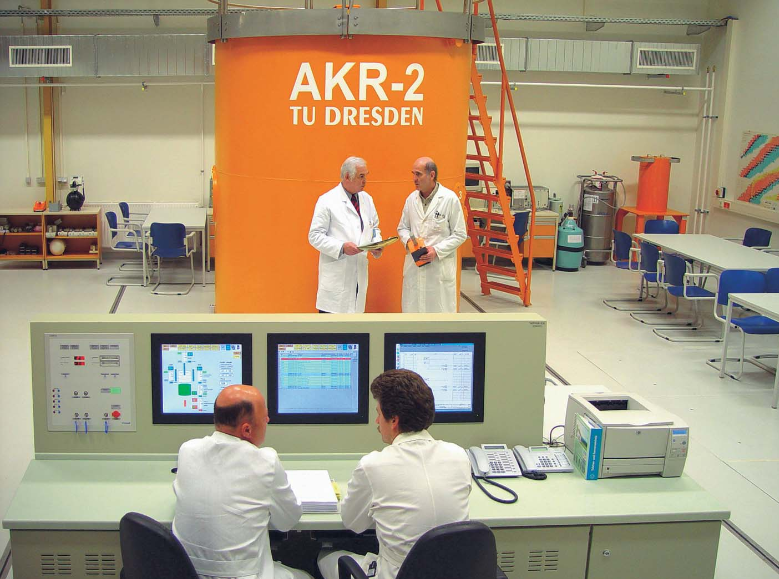
\includegraphics[width=0.7\textwidth]{pic/akr2.png}\\
				\text{\tiny{Quelle: TUD Institut für Energietechnik. \textit{AKR-2 Bau und Inbetriebnahme}, Dresden. Juli 2005}}
			\end{figure}	
	\end{frame}

	\begin{frame}{AKR-2: Aufbau und Maßnahmen zur nuklearen Sicherheit}
		\begin{figure}[ht]
			\centering
			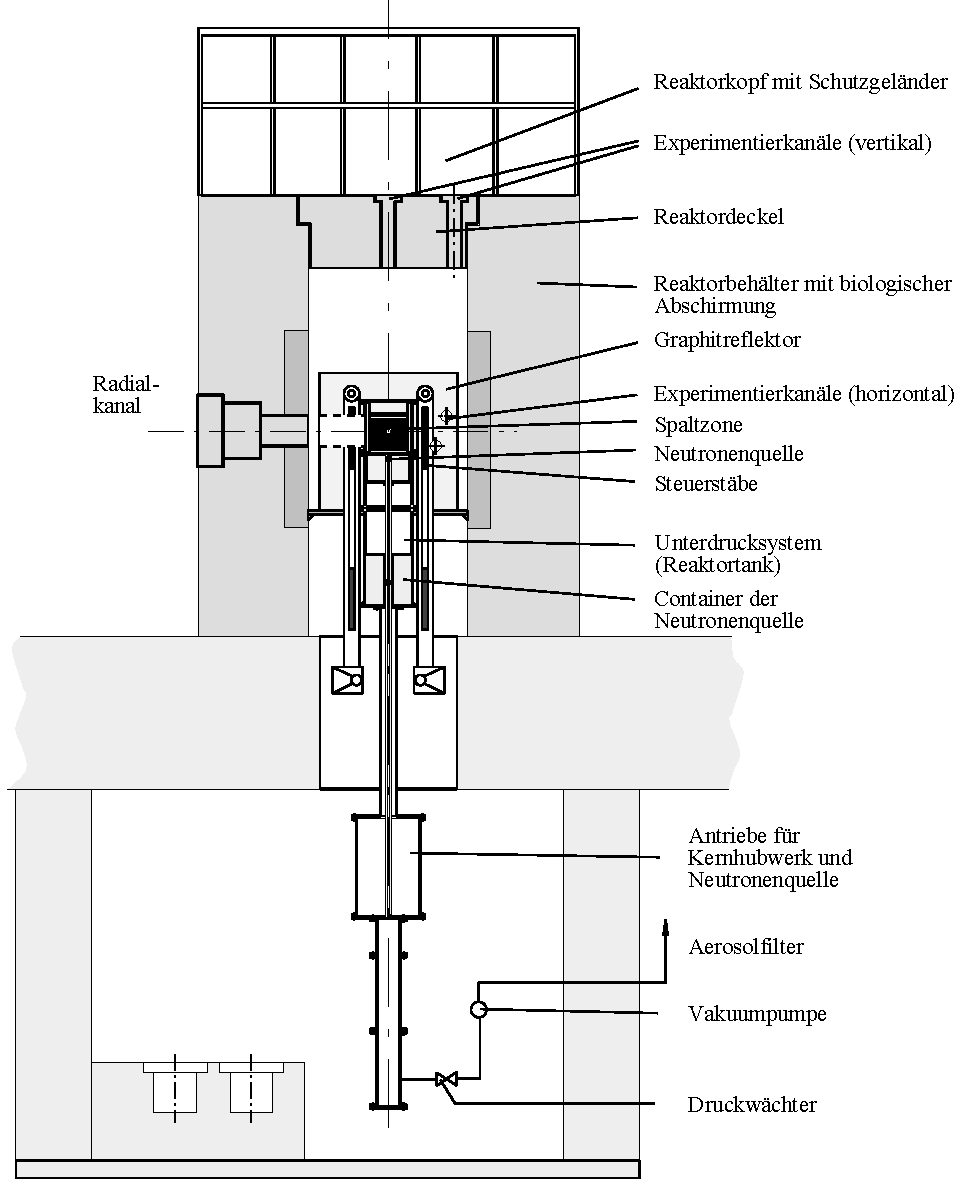
\includegraphics[width=0.5\textwidth]{pic/Vertikalquerschnitt_Reaktor.pdf}\\
			\text{\tiny{Quelle: TUD Institut für Energietechnik. \textit{AKR-2 Bau und Inbetriebnahme}, Dresden. Juli 2005}}
		\end{figure}	
	\end{frame}
	
	\begin{frame}{AKR-2: Aufbau und Maßnahmen zur nuklearen Sicherheit}
			\begin{figure}[ht]
				\centering
				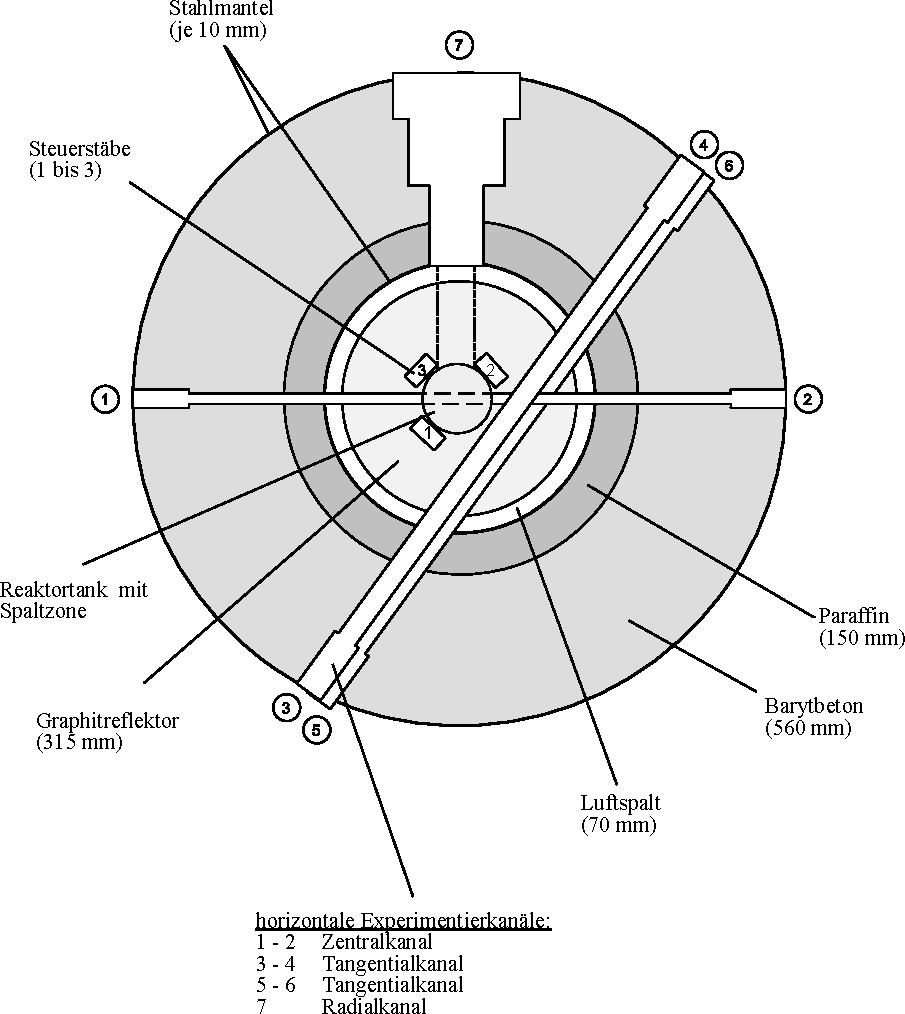
\includegraphics[width=0.5\textwidth]{pic/Horizontalquerschnitt_Reaktor}\\
				\text{\tiny{Quelle: TUD Institut für Energietechnik. \textit{AKR-2 Bau und Inbetriebnahme}, Dresden. Juli 2005}}
			\end{figure}	
	\end{frame}

\end{document}